\section{Task 2: analysis of numerical methods}

\subsection{Method overview and problem}
This task analyzes bisection, false position, Newton--Raphson and secant methods for finding function roots. Each is described in terms of assumptions, formula derivation and implementation.

\subsubsection{Bisection method}
Bisection is one of the simplest numerical root-finding methods.

\begin{itemize}
    \item Assumptions:
    \begin{itemize}
        \item \( f(x) \) is continuous on \([a, b]\).
        \item At least one root exists in \([a, b]\), that is, \( f(a) \cdot f(b) < 0 \).
    \end{itemize}
    \item Formula:
    \[ c = \frac{a + b}{2} \]
    \item Derivation:
    Repeatedly bisect \([a, b]\). At each step, select the subinterval containing a root using the sign of \( f(a) \cdot f(c) \). Continue until the desired accuracy \( \text{acc} \) is reached.
\end{itemize}

\subsubsection{False-position method}
False position uses a line to find roots from function values at interval endpoints.

\begin{itemize}
    \item Assumptions:
    \begin{itemize}
        \item \( f(x) \) is continuous on \([z_1, z_2]\).
        \item \( f(z_1) \cdot f(z_2) < 0 \).
    \end{itemize}
    \item Formula:
    \[ c = \frac{a \cdot f(b) - b \cdot f(a)}{f(b) - f(a)} \]
    \item Derivation:
    Approximate a root using the line through \((a, f(a))\) and \((b, f(b))\). The next point \( c \) is its intersection with the \( x \)-axis ($f(c) = 0$).
    \[
     \frac{-f(a)}{c-a} = \frac{f(c) - f(a)}{c-a} = \frac{f(b) - f(a)}{b-a}
    \]
    Rearrangement gives:
    \[ c = \frac{a \cdot f(b) - b \cdot f(a)}{f(b) - f(a)} \]
    Repeat until the difference between successive approximations reaches the desired accuracy.
\end{itemize}

\subsubsection{Newton--Raphson method}
Newton--Raphson is a fast iterative method using function derivatives.

\begin{itemize}
    \item Assumptions:
    \begin{itemize}
        \item \( f(x) \) is differentiable near the root.
        \item A starting point \( x_0 \) near the root is known.
    \end{itemize}
    \item Formula:
    \[ x_{i+1} = x_i - \frac{f(x_i)}{f'(x_i)} \]
    \item Derivation:
    Expand the function in a Taylor series at \( x_i \).
    \[
    f(x) \sim f(x_0) + f'(x_0)(x - x_0) 
    \]
    Rearranging and assuming $(f(x) = 0)$ gives:
    \[
    x = x_0 - \frac{f(x_0)}{f'(x_0)}
    \]
    The tangent at \( x_i \) intersects the \( x \)-axis at the next approximation \( x_{i+1} \). Iterate until \( |f(x_{i+1})| < \text{acc} \).
\end{itemize}

\subsubsection{Secant method}
The secant method modifies Newton--Raphson so that derivatives need not be computed.

\begin{itemize}
    \item Assumptions:
    \begin{itemize}
        \item \( f(x) \) need not be differentiable.
        \item Two starting points \( x_0 \) and \( x_1 \) are known.
    \end{itemize}
    \item Formula:
    \[ x_{i+1} = x_i - \frac{f(x_i)(x_i - x_{i-1})}{f(x_i) - f(x_{i-1})} \]
    \item Derivation:
    Replace the tangent with the secant through successive points \((x_{i-1}, f(x_{i-1}))\) and \((x_i, f(x_i))\). Expand the derivative using its definition and substitute the corresponding values.
\end{itemize}

\subsection{Tests}
Two test types were performed for each method:

\begin{itemize}
    \item Error versus iteration count, for ranges (2-20 and 2-120).
    \item Iteration count and runtime needed for a specified accuracy \(\in [10^{-1}, 10^{-32}\). Maximum iteration count $=1000$.
\end{itemize}

Test functions:\\
\begin{itemize}
    \item \( \text{Pol } x=0.23 \): \( f(x) = (x - 0.23)(x + 1)(x + 2)(x + 3)(x + 4) \)
    \item \( \text{Pol } x=0.53 \): \( f(x) = (x - 0.53)(x + 1)(x + 2)(x + 3)(x + 4) \)
\end{itemize}
For each function, we considered starting points nearer the center of the interval and nearer an endpoint.

{\centering
\paragraph{Error growth}
\indent

\paragraph{Interval \([0, 1]\)}
\indent

\begin{minipage}{0.48\textwidth}
    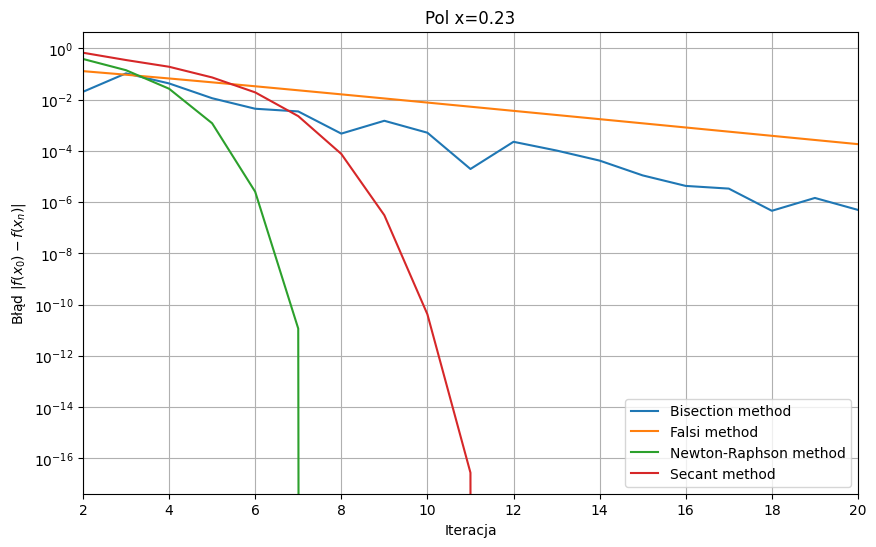
\includegraphics[width = \textwidth]{figures/task-2error_rising/0_1/20_x_0_23.png}
\end{minipage}
\begin{minipage}{0.48\textwidth}
    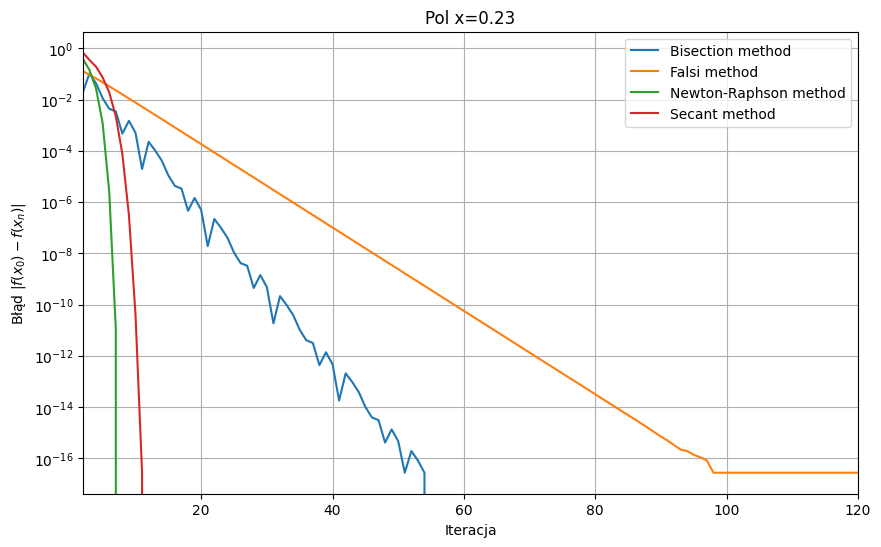
\includegraphics[width = \textwidth]{figures/task-2error_rising/0_1/120_x_0_23.png}
\end{minipage}
Polynomial with $x_0 = 0.23$

\begin{minipage}{0.48\textwidth}
    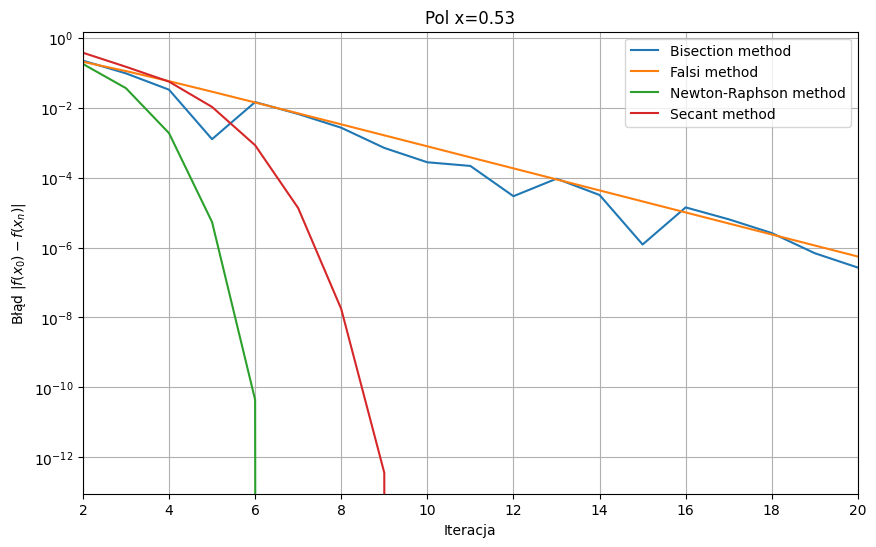
\includegraphics[width = \textwidth]{figures/task-2error_rising/0_1/20_x_0_53.png}
\end{minipage}
\begin{minipage}{0.48\textwidth}
    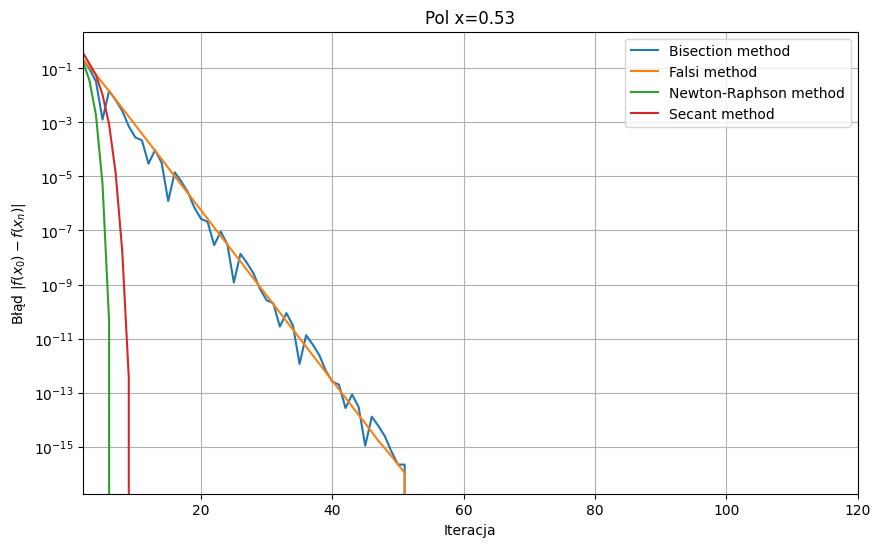
\includegraphics[width = \textwidth]{figures/task-2error_rising/0_1/120_x_0_53.png}
\end{minipage}
Polynomial with $x_0 = 0.53$

\paragraph{Interval \([0, 100]\)}
\indent

\begin{minipage}{0.48\textwidth}
    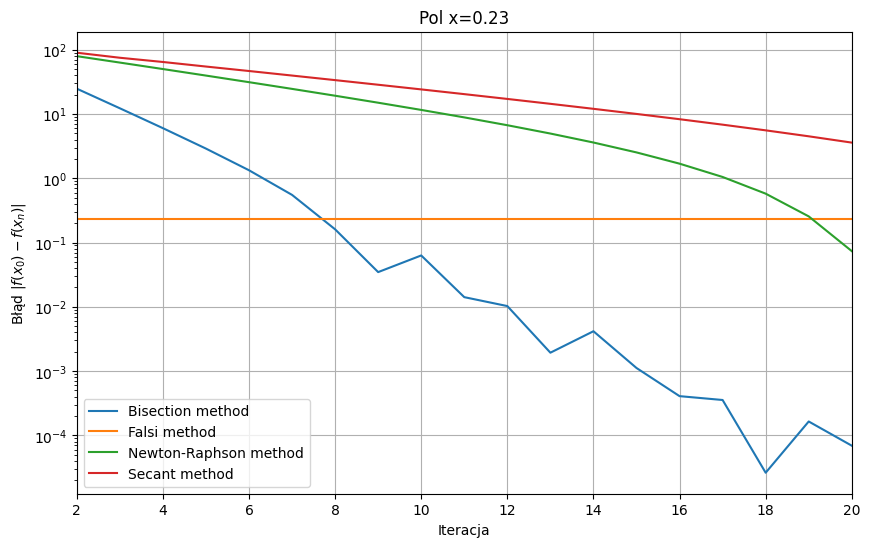
\includegraphics[width = \textwidth]{figures/task-2error_rising/0_100/20_x_0_23.png}
\end{minipage}
\begin{minipage}{0.48\textwidth}
    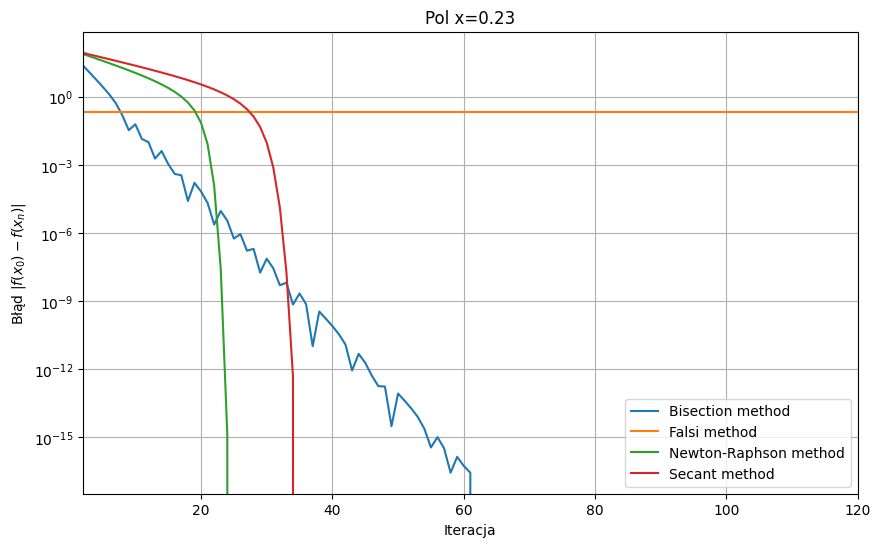
\includegraphics[width = \textwidth]{figures/task-2error_rising/0_100/120_x_0_23.png}
\end{minipage}
Polynomial with $x_0 = 0.23$

\begin{minipage}{0.48\textwidth}
    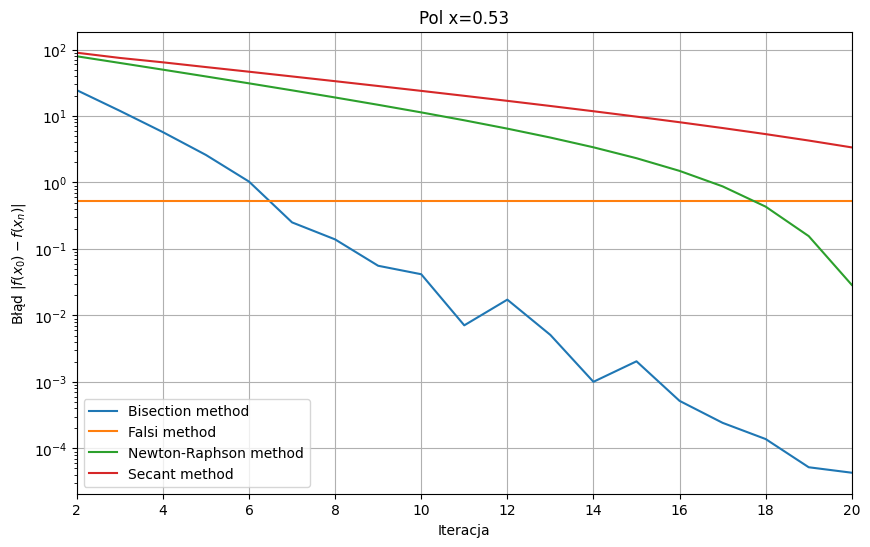
\includegraphics[width = \textwidth]{figures/task-2error_rising/0_100/20_x_0_53.png}
\end{minipage}
\begin{minipage}{0.48\textwidth}
    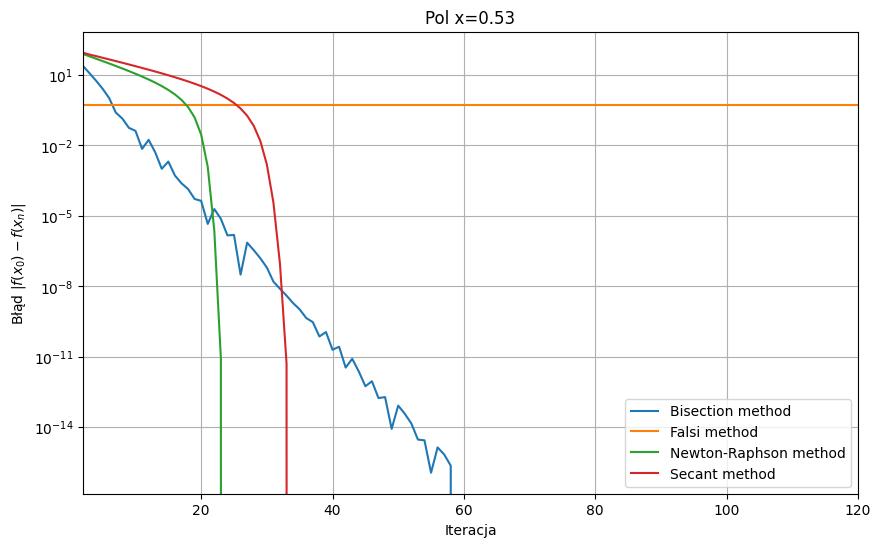
\includegraphics[width = \textwidth]{figures/task-2error_rising/0_100/120_x_0_53.png}
\end{minipage}
Polynomial with $x_0 = 0.53$

}

{\centering
\paragraph{Attaining the required accuracy}
\indent

\paragraph{Interval \([0, 1]\)}
\indent

\begin{minipage}{0.48\textwidth}
    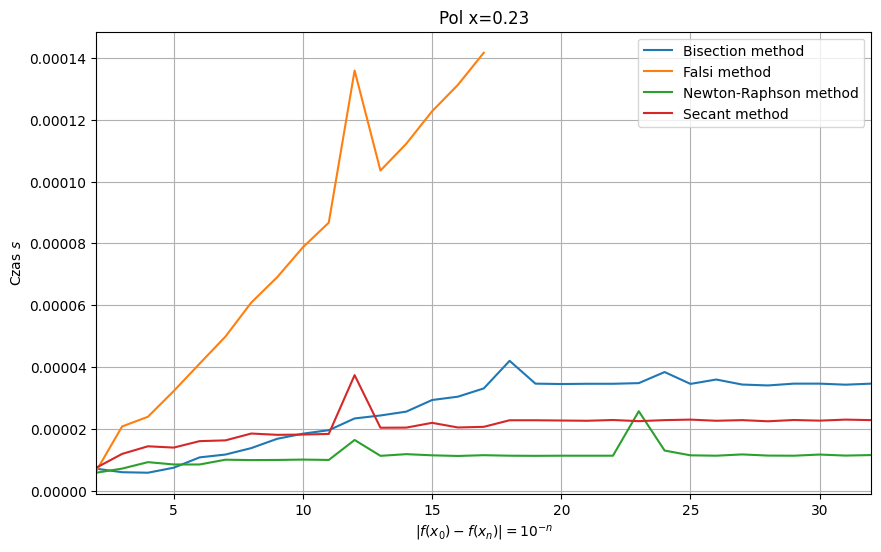
\includegraphics[width = \textwidth]{figures/task-2accuracy_till/0_1/time_023.png}
\end{minipage}
\begin{minipage}{0.48\textwidth}
    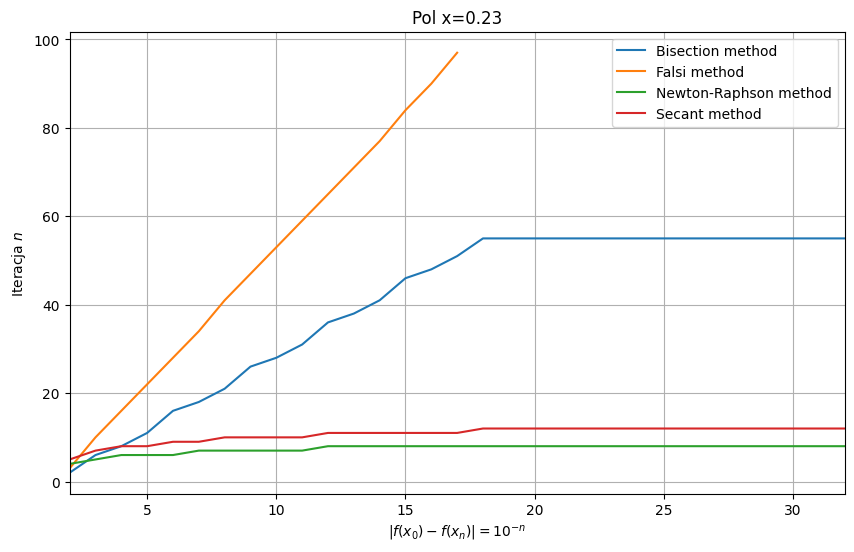
\includegraphics[width = \textwidth]{figures/task-2accuracy_till/0_1/iteration_023.png}
\end{minipage}
Polynomial with $x_0 = 0.23$

\begin{minipage}{0.48\textwidth}
    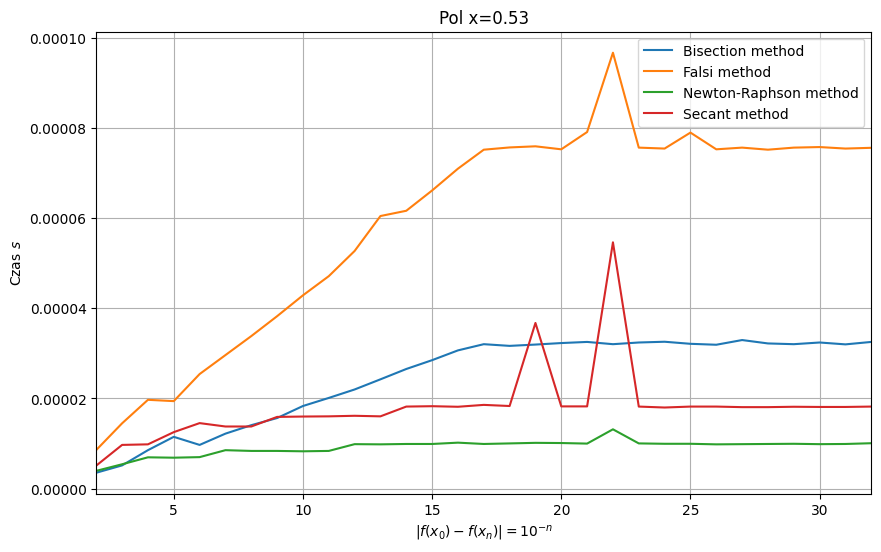
\includegraphics[width = \textwidth]{figures/task-2accuracy_till/0_1/time_053.png}
\end{minipage}
\begin{minipage}{0.48\textwidth}
    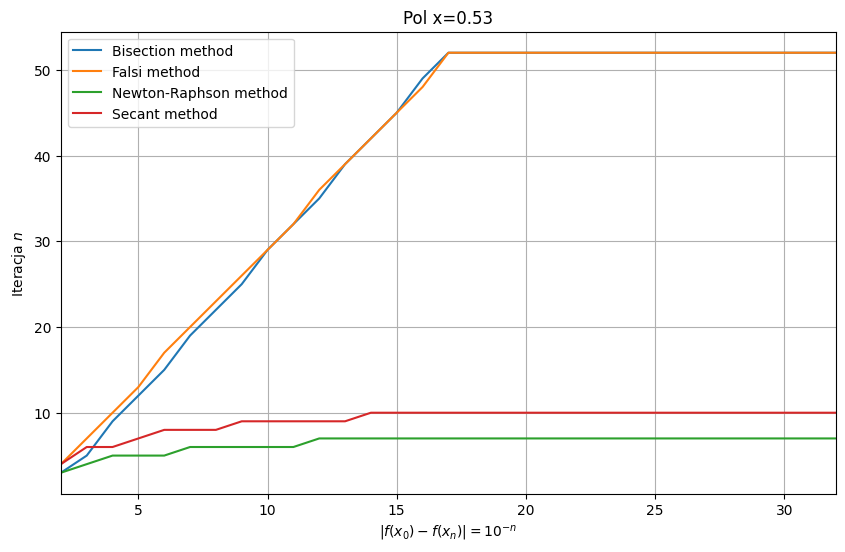
\includegraphics[width = \textwidth]{figures/task-2accuracy_till/0_1/iteration_053.png}
\end{minipage}
Polynomial with $x_0 = 0.53$

\paragraph{Interval \([0, 100]\)}
\indent

\begin{minipage}{0.48\textwidth}
    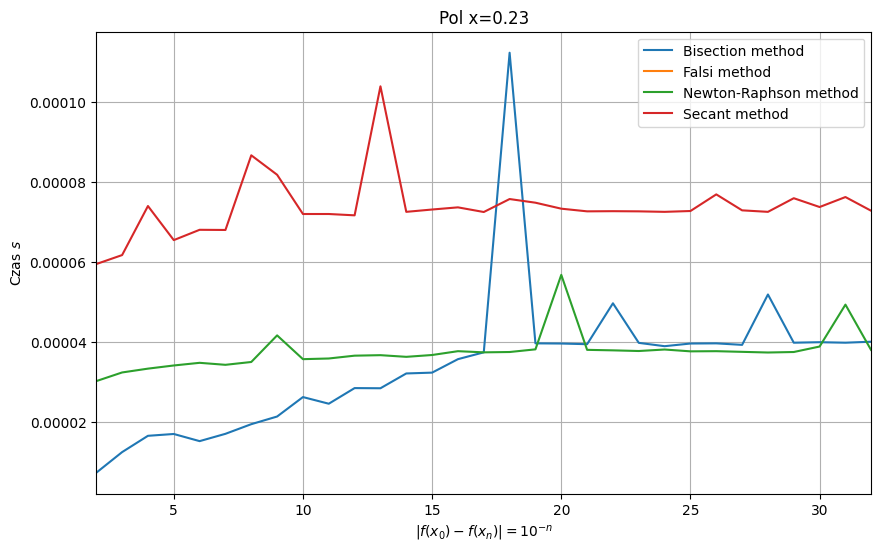
\includegraphics[width = \textwidth]{figures/task-2accuracy_till/0_100/time_023.png}
\end{minipage}
\begin{minipage}{0.48\textwidth}
    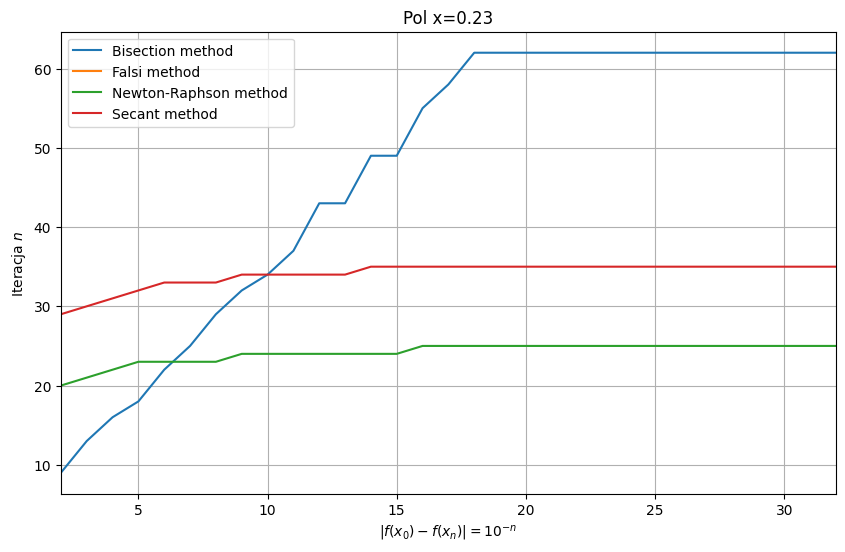
\includegraphics[width = \textwidth]{figures/task-2accuracy_till/0_100/iteration_023.png}
\end{minipage}
Polynomial with $x_0 = 0.23$

\begin{minipage}{0.48\textwidth}
    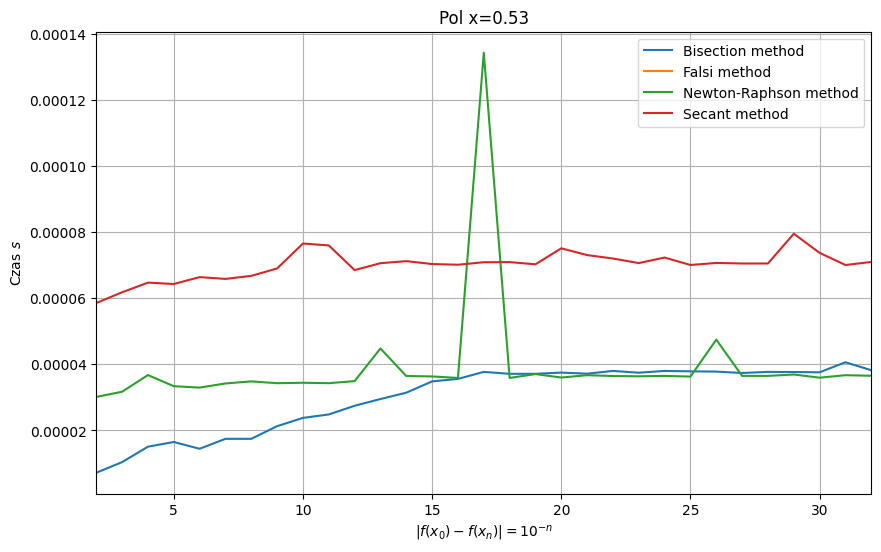
\includegraphics[width = \textwidth]{figures/task-2accuracy_till/0_100/time_053.png}
\end{minipage}
\begin{minipage}{0.48\textwidth}
    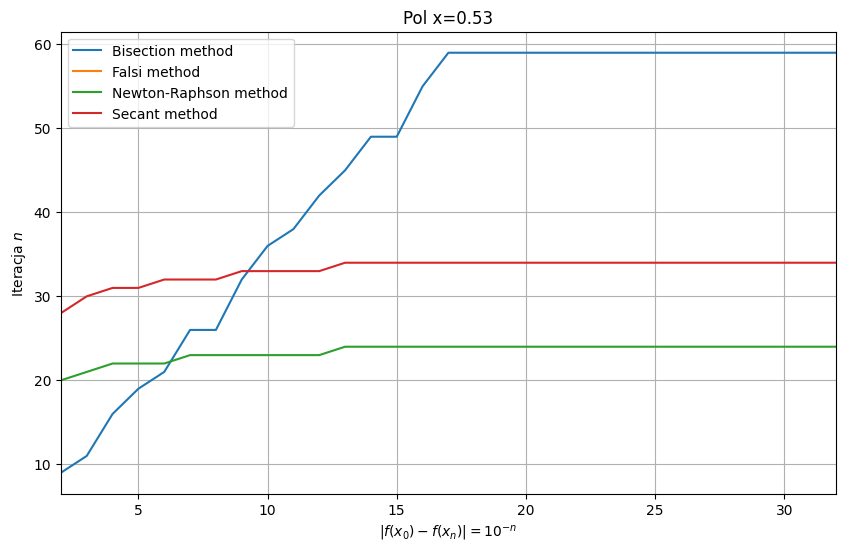
\includegraphics[width = \textwidth]{figures/task-2accuracy_till/0_100/iteration_053.png}
\end{minipage}
Polynomial with $x_0 = 0.53$

}


\subsection{Conclusions and analysis}
\paragraph{Error versus iteration count}
\begin{itemize}
\item Newton--Raphson is fastest, although it requires an initial point near the root. Its error decreases exponentially, making it very efficient.
\item The secant method is slower than Newton--Raphson but permits approximation of nondifferentiable functions. Its accuracy also increases exponentially, with a smaller convergence coefficient.
\item False position reduces error linearly but is ineffective for roots extremely close to an endpoint. Its runtime is worse than or comparable with bisection. The test functions may have been particularly unsuitable for this method, which proposes a statistical solution and should be more efficient.
\end{itemize}

\paragraph{Iterations and runtime needed to reach the target precision}
\begin{itemize}
\item For bisection and false position, runtime and iteration count grow linearly with the required precision.
\item For Newton--Raphson and the secant method, iteration count and runtime are constant once the root is reached.
\item Over a large interval, false position was inefficient and sometimes did not converge, making it unusable in those cases.
\end{itemize}

